\documentclass{book}
% comment out the following line if you want to latex the whole book:
%\includeonly{ch9}
  % preamble

\usepackage{verbatim}\usepackage{epsf}

\setlength{\textwidth}{5.2in}            % default seems to be around 4.8 inch,
\addtolength{\evensidemargin}{-0.2in}    % so we can devide the extra 0.4 inch
\addtolength{\oddsidemargin}{-0.2in}     % equally over left and right margin

\setlength{\parindent}{2.5em}
\setlength{\parskip}{1.2 ex plus0.2ex minus 0.1ex}
\renewcommand{\baselinestretch}{1.05}
\renewcommand{\floatpagefraction}{1.0}
\renewcommand{\topfraction}{1.0}

\begin{document}
  \frontmatter
\makebox[3.5in][s]{}\verb=Time-stamp: <2002-04-12 13:25:12 piet>=
%
% nice latex feature: you can specify which files you want to include in your
% next output, by listing only those files as arguments to \includeonly{} 
% above on the third line (I had to put this comment here, since the emacs
% time stamp is only recognized in the first eight lines).
% NOTE: if you want to print out the whole book, simply comment out the line
% starting with \includeonly above.
%
% It is a good idea to write this top level file out, each time a change has
% been made, in order to get the correct time stamp to appear on the title
% page.  Even if you print out only one chapter, still the title page will
% appear, so that the time stamp will be include (otherwise the time stamp
% would appear uselessly on a separate white page, before the chapter).
%
    \def\half{{\ifmmode{{1 \over 2}}\else{${1 \over 2}$}\fi}}
\def\dhalf{{\textstyle {1 \over 2}}}
\def\threehalf{{\ifmmode{{3 \over 2}}\else{${3 \over 2}$}\fi}}
\def\dthreehalf{{\textstyle {3 \over 2}}}
\def\dfivehalf{{\textstyle {5 \over 2}}}
\def\dfivethree{{\textstyle {5 \over 3}}}
\def\bx{{\bf x}}
\def\br{{\bf r}}
\def\bv{{\bf v}}
\def\ba{{\bf a}}
\def\bj{{\bf j}}
\def\bs{{\bf s}}
\def\bc{{\bf c}}
\def\bp{{\bf p}}
\def\bk{{\bf k}}
\def\badot{{\bf \dot a}}
\def\batwo{{{\bf  a}^{(2)}}}
\def\bathree{{{\bf  a}^{(3)}}}
\def\bR{{\bf R}}
\def\bV{{\bf V}}
           % input, not include, since all files need the \def{}
    % title page

\thispagestyle{empty}                 % suppresses page numbering of first page

\begin{latexonly}

\begin{center}


\hbox{}

\bigskip\bigskip


{\lggggb Moving Stars Around}

\bigskip


\bigskip\bigskip


{\lggb A Preliminary Version}


\medskip


{\lggb of what will expand into}


\medskip

{\lggb Volumes 1,2,3}

\medskip

{\lggb of the series}

\bigskip\bigskip

{\lgggb The Art of Computational Science}

\bigskip\bigskip

\end{center}

\end{latexonly}


\begin{htmlonly}


\begin{center}


\hbox{}

\bigskip\bigskip


{\huge \bf Moving Stars Around}

\medskip


{\LARGE A Preliminary Version}



{\LARGE of what will expand into}


\medskip



{\LARGE Volumes 1,2,3}

\medskip



{\LARGE of the series}


\bigskip


{\huge \bf The Art of Computational Science}



\bigskip


\end{center}
\end{htmlonly}

 \begin{latexonly}
 \begin{center}
 \leavevmode
 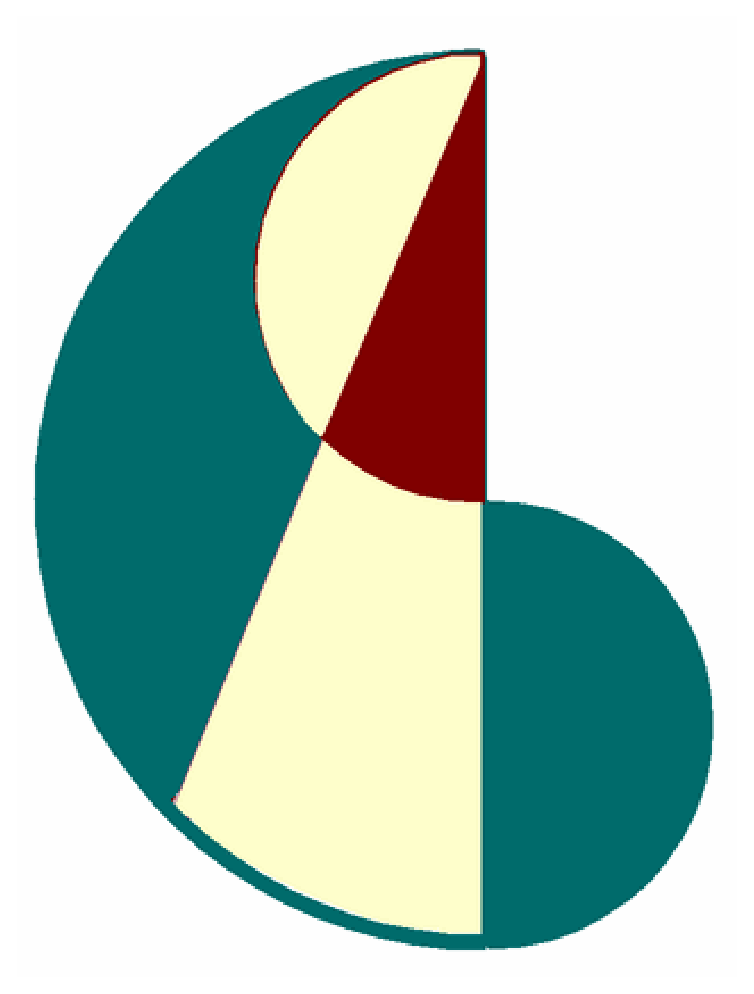
\includegraphics[width=4cm]{acstitle.eps}
 \end{center}
 \end{latexonly}


\begin{htmlonly}
\begin{center}
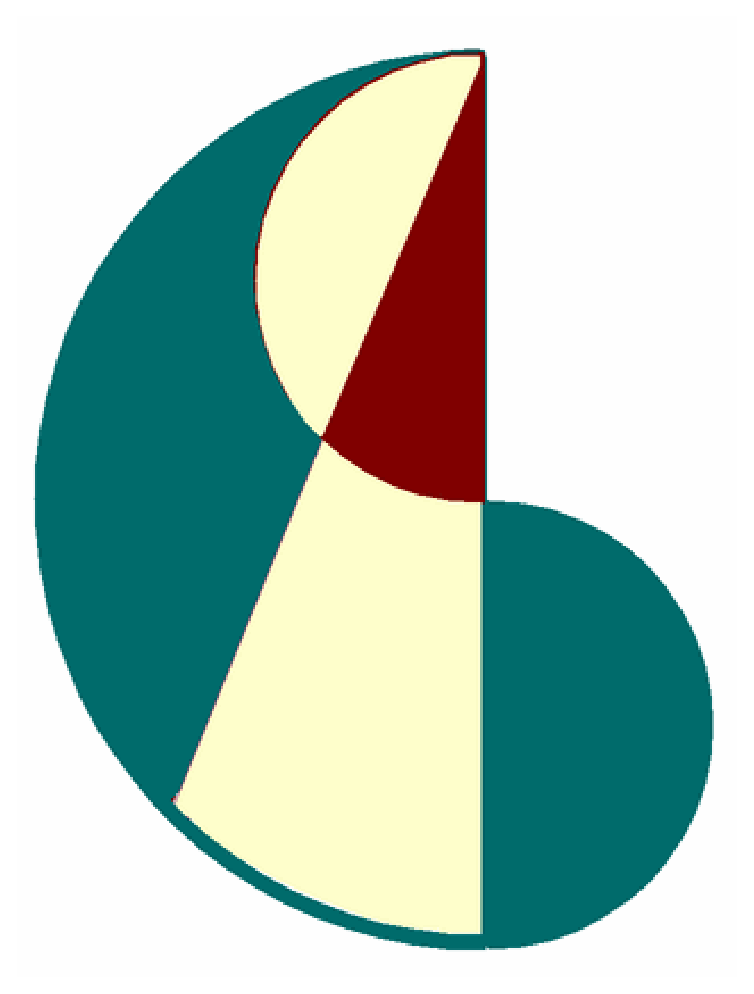
\includegraphics[width=3cm]{acstitle.eps}
\end{center}
\end{htmlonly}

\bigskip\bigskip\bigskip


\begin{center}
% lggr -> Large
% lr -> large
\begin{tabular}{llllllll}
& {\LARGE Piet Hut} & {\LARGE \&} & & & & & {\LARGE Jun Makino}\\
&  & & & & & & \\
& {\large Institute for Advanced Study} & & & & & &
  {\large Univ. of Tokyo, \ Dept. of Astronomy}\\
& {\large 1 Einstein Drive} & & & & & & {\large 7-3-1 Hongo, Bunkyo-ku}\\
& {\large Princeton, NJ 08540} & & & & & & {\large Tokyo 113-0033}\\
& {\large U.S.A.} & & & & & & {\large JAPAN}\\
& {\large piet@ias.edu} & & & & & & {\large makino@astron.s.u-tokyo.ac.jp}\\
\end{tabular}

\bigskip\bigskip\bigskip\bigskip

\end{center}
         % input, in order to let the time stamp appear
%
% uncomment the following three lines, if you want to print two pages
% on one, using e.g. "psnup -2 v1.ps > v1_2.ps".  Normally the next three
% lines should be commented out, but in that case psnup will print the right
% (left) pages on the left (right) side.
%
%\newpage
%\thispagestyle{empty}
%\mbox{}
%
    \newpage           % blank page, to force preface to start on a right hand page
\thispagestyle{empty}      % suppresses page numbering of the blank second page
\mbox{}                    % dummy content; otherwise \newpage has no effect
\newpage                   % on to third page, to start the preface
\pagenumbering{roman}      % with a roman numbering system, starting here at i

%%\chapter{Preface} %% this replace the four lines below, but at the
                    %% cost (currently) of two extra pages

\addcontentsline{toc}{chapter}{Preface}

\begin{center}
{\lgb Preface}
\end{center}

The {\it Pure Gravity} book series, of which this is the second volume,
\dots\dots\dots

%\bigskip
%\bigskip
%{\it Acknowledgments:}
%xxx
%We thank xxx, xxx and xxx for valuable
%discussions.  This work is supported in part by the Research for the
%Future Program of Japan Society for the Promotion of Science
%(JSPS-RFTP97P01102).

\tableofcontents

\listoffigures


  \mainmatter
      \chapter{Gravitational Scattering Experiments}


    \part{3-Body Scattering in 1D}
      \chapter{Regularization}


      \chapter{Setting Up and Analyzing Gravitational Scattering Experiments}


      \chapter{A Topological Investigation of Parameter Space}


    \part{3-Body Scattering in 2D}
      \chapter{Levi-Civita Regularization}


      \chapter{Cross Sections and Reaction Rates}


    \part{3-Body Scattering in 3D}
      \chapter{Quaternion Regularization}


      \chapter{Cross Sections and Reaction Rates}


      \chapter{A Watershed in Energy Flow}


    \part{Many-Body Scattering}
      \chapter{The Many Channels in 4-Body Scattering}


      \chapter{A General Scattering Code}


      \chapter{Astrophysical Applications}


%    \appendix
%      \addcontentsline{toc}{part}{Appendices}

\chapter{yyyy}


%      \chapter{zzzz}


  \backmatter
\end{document}
%
% ...........................................................................
%
% history:
%
% May 2001: ph and jm met in New York, where they wrote code and produced
%           pictures for the two-body problem.
%
% July 2001: ph and jm met in Tokyo, where they wrote code and produced
%            pictures for the figure-8 three-body problem.
%
% Nov. 2001: ph and jm met in New York, where they discussed how to structure
%            the first three volumes.  Following their meeting, ph started to
%            write draft text for the first part of volume 1.
%
% Dec. 2001: ph started to add introductory text in preface and early chapters
%            and ph and jm began to experiment with joint code development and
%            text writing across the internet
%
% ...........................................................................
%
